%%%%%%%%%%%%%%%%%%%%%%%%%%%%%%%%%%%%%%%%%
% Short Sectioned Assignment
% LaTeX Template
% Version 1.0 (5/5/12)
%
% This template has been downloaded from:
% http://www.LaTeXTemplates.com
%
% Original author:
% Frits Wenneker (http://www.howtotex.com)
%
% License:
% CC BY-NC-SA 3.0 (http://creativecommons.org/licenses/by-nc-sa/3.0/)
%
%%%%%%%%%%%%%%%%%%%%%%%%%%%%%%%%%%%%%%%%%

%----------------------------------------------------------------------------------------
%	PACKAGES AND OTHER DOCUMENT CONFIGURATIONS
%----------------------------------------------------------------------------------------

\documentclass[letterpaper, fontsize=12pt]{scrartcl} % A4 paper and 11pt font size

\usepackage[T1]{fontenc} % Use 8-bit encoding that has 256 glyphs
\usepackage{fourier} % Use the Adobe Utopia font for the document - comment this line to return to the LaTeX default
\usepackage[english]{babel} % English language/hyphenation
\usepackage{amsmath,amsfonts,amsthm} % Math packages

\usepackage{lipsum} % Used for inserting dummy 'Lorem ipsum' text into the template
\usepackage[margin=1in]{geometry} %set margins -TA
\usepackage{sectsty} % Allows customizing section commands
\allsectionsfont{\centering \normalfont\scshape} % Make all sections centered, the default font and small caps
\usepackage{enumitem}
\usepackage{fancyhdr} % Custom headers and footers
\usepackage{graphicx}
\usepackage{float}

\usepackage{graphicx} % Required to insert images
\usepackage{multicol}
\usepackage{enumitem}
\usepackage{amssymb}
\usepackage{bm}
\usepackage{verbatim}
\usepackage{hyperref}
\usepackage{color}
\usepackage[]{mcode} %MATLAB code

\allowdisplaybreaks


\pagestyle{fancyplain} % Makes all pages in the document conform to the custom headers and footers
\fancyhead{} % No page header - if you want one, create it in the same way as the footers below
\fancyfoot[L]{\textit{CME 102 Fall '17-'18}} % Empty left footer
\fancyfoot[C]{\thepage} % Empty center footer
\fancyfoot[R]{Tim Anderson} % Page numbering for right footer
\renewcommand{\headrulewidth}{0pt} % Remove header underlines
\renewcommand{\footrulewidth}{0pt} % Remove footer underlines
\setlength{\headheight}{0pt} % Customize the height of the header
\setlength{\footheight}{0pt} % Customize the height of the header

\numberwithin{equation}{section} % Number equations within sections (i.e. 1.1, 1.2, 2.1, 2.2 instead of 1, 2, 3, 4)
\numberwithin{figure}{section} % Number figures within sections (i.e. 1.1, 1.2, 2.1, 2.2 instead of 1, 2, 3, 4)
\numberwithin{table}{section} % Number tables within sections (i.e. 1.1, 1.2, 2.1, 2.2 instead of 1, 2, 3, 4)

\setlength\parindent{0pt} % Removes all indentation from paragraphs - comment this line for an assignment with lots of text
\begin{document}

%----------------------------------------------------------------------------------------
%	TITLE SECTION
%----------------------------------------------------------------------------------------

\newcommand{\horrule}[1]{\rule{\linewidth}{#1}} % Create horizontal rule command with 1 argument of height

%---------------------------------------------------------------------------------------a-
%	PROBLEM 1
%----------------------------------------------------------------------------------------

\section*{Midterm \#1 Review Problems}
\par If not otherwise specified, solve the following problems. If initial conditions are given, solve for all constants of integration. It is okay to leave answers in implicit form or with unsolved integrals if it is not possible to reduce the solution further. 

\begin{enumerate}


\item \textbf{Separation of variables}
\begin{enumerate}[label = (\alph*)]
% Kreyszig 1.3 #3
\item $y ' = \sec^2 y$

%\par \textbf{Solution:}
%\begin{align*}
%y' &= \sec^2( y) \\
%\cos^2(y)dy &= dx \\
%\frac{1}{2} (1 + \cos(2y))dy &= dx \\
%\frac{y}{2} + \frac{1}{4} \sin(2y) &= x + C \quad\blacksquare
%\end{align*}

% Kreyszig 1.3 #8 
\item $y' = (y + 4x)^2$

%\par \textbf{Solution:}
%\begin{align*}
%y' &= (y + 4x)^2 \\
%v &= y + 4x \\
%v' &= y' + 4 \\
%v' - 4 &= v^2 \\
%v' &= v^2 + 4 \\
%\frac{dv}{v^2 + 4} &= dx \\
%\frac{1}{2} \tan \left( \frac{v}{2}\right) &= x + C \\
%v &= 2\tan^{-1}(2x + C) \\
%y &= 2\tan^{-1}(2x + C) - 4x \quad\blacksquare 
%\end{align*}

% Kreyszig 1.3 #10
\item $xy' = x + y$

%\par \textbf{Solution:}
%\begin{align*}
%xy' &= x + y \\
%y' &= 1 + \frac{y}{x} \\
%v &= \frac{y}{x} \\
%y &= xv \\
%y' &= v + x v' \\
%v + x v' &= 1 + v \\
%v' &= \frac{1}{x} \\
%v &= \ln(x) + C\\
%y &= x(\ln(x) + C) \quad\blacksquare
%\end{align*}

\end{enumerate}


\item \textbf{Equilibrium solutions} 
\begin{enumerate}[label = (\alph*)]
\item Find and characterize the equilibria for $y' = (y^2-7y + 10)(y^2 + 4y + 4)$. 

%\par \textbf{Solution:} we first factor $y'$ to find $y' = (y-5)(y-2)(y+2)^2$. From here, we find that $y = 5, 2, \; -2$ are the equilibrium solutions since these are the zeros $y'$. (Remember that to even have equilibrium solutions, the system needs to be \textit{autonomous} i.e. $y'$ cannot depend on $x$.) 
%
%\par To characterize the solutions, we pick test points in between and outside the zeros. These test points will tell us the sign of the derivative between the equilibria. We can use the sign of the derivative to determine the stability of each solution. To do this, we pick $ y = -3, 0, 3, 6$ as test points:
%
%\begin{align*}
%y'(-3) &= (-3 -5)(-3-2)(-3+2)^2 > 0 \\
%y'(0) &= (-5)(-2)(2)^2 >0 \\
%y(3) &= (3 -5)(3-2)(-3+2)^2 < 0 \\
%y(6) &= (6 - 5)(6 - 2)(6 + 2)^2 > 0 
%\end{align*}
%
%So, we know that $y = -2$ is semistable, $y = 2$ is stable, and $y = 5$ is unstable. 

%\item In the following direction field, identify and characterize the equilibrium solutions. 
%\begin{figure}[H]
%\centering \includegraphics[width=0.5\columnwidth]{midterm1review_1.png}
%\end{figure}
%
%\par \textbf{Solution:}


\end{enumerate}

\item \textbf{Linear 1st order ODE and related topics}
\begin{enumerate}[label = (\alph*)]
% Kreyszig 1.4 #4
\item $y = 2y - 4x$
%
%\par \textbf{Solution:} This is a linear first order inhomogeneous ODE, and we know that we have a nice closed form solution we can just plug and chug with:
%\begin{align*}
%y(x) &= e^{-\int p(x) dx} \left[ \int r(x) e^{\int p(x) dx} dx + C\right]
%\end{align*}

% Kreyszig 1.4 #11
\item $y' = (y-2)\cot(x)$

%\par \textbf{Solution:} This is also a linear first order inhomogeneous ODE, so we can just plug and chug with the solution we derived in class:
%\begin{align*}
%y(x) &= e^{-\int p(x) dx} \left[ \int r(x) e^{\int p(x) dx} dx + C\right] \\
%&=  e^{-\int -\cot(x) dx} \left[ \int -2\cot(x) e^{\int -\cot(x) dx} dx + C\right] \\
%&= e^{ \ln(\sin(x))} \left[ \int -2\cot(x) e^{-\ln(\sin(x)) dx} dx + C\right] \\
%&= \sin(x) \left[ \int -2\cot(x) \csc(x) dx + C\right] \\
%&= \sin(x) \left[ 2\csc(x) + C\right]\\
%&= 2 + C\sin(x) \quad\blacksquare
%\end{align*}

% Kreyszig 2.9 #1
\item Derive the equation for the following circuit and find the current $I(t)$ where $E(t) = e^{-t}$ i.e. a constant voltage, $R = C = 1$, and $I(0) = 0$: 

\begin{figure}[H]
\centering 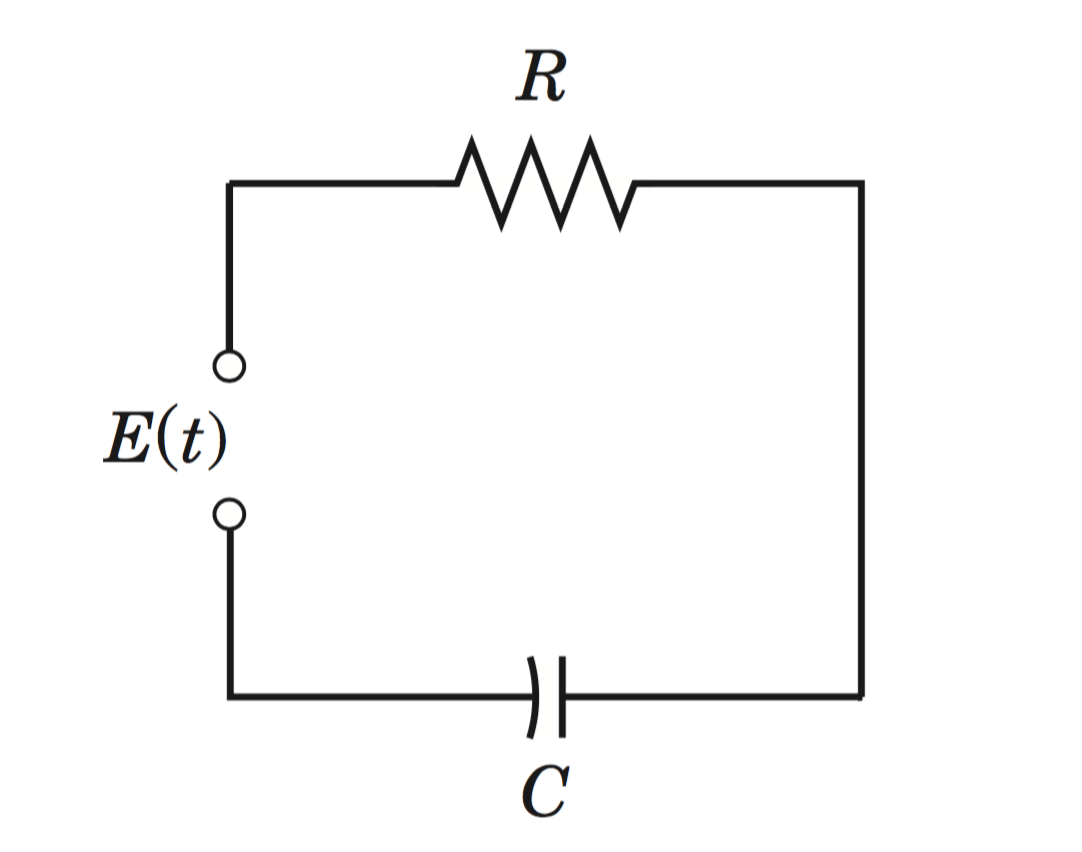
\includegraphics[width=0.5\columnwidth]{midterm1review_circuit.png}
\end{figure}

%\par \textbf{Solution:} We derive the ODE using Kirchoff's voltage law:
%\[ \sum_i V_i = E(t) - RI - \frac{Q}{C} = e^{-t} - I - \int_0^\tau I(\tau) d\tau = 0 \]
%We can take the derivative of both sides to find:
%\[ I' + I = - e^{-t} \]
%
%This ODE is just a linear first order inhomogeneous ODE which we can easily solve:
%\begin{align*}
%I' + I &= - e^{-t} \\
%I(t) &= e^{-\int dt}\left[ \int -e^{-t} e^{\int dt} dt + C\right] \\
%&= e^{-t} \left[ \int - e^{-t} e^t dt + C\right] \\
%&= e^{-t} \left[ -t + C\right] \\
%I(0) &= 0 = C \\
%I(t) &= -e^{-t} \quad\blacksquare
%\end{align*}

\item Solve: $y' + y = -x/y$

%\par \textbf{Solution:} You should immediately identify that this is a Bernoulli equation. We can substitute $u = y^{1 - \alpha} = y^2$ and solve for $u$:
%\begin{align*}
%u& = y^2\\
%u' &= 2yy' \\
%y' + y &=  -x/y\\
%\intertext{Multiplying through by $y$ (since we know we need $yy'$ and $y^2$ to appear somewhere in the equation so we can make the substitution):}
%yy' + y^2 &= -x\\
%\frac{1}{2} u' + u &= -x \\
%u' + 2u &= -2x \\
%u(x) &= e^{-\int 2dx} \left[ \int (-2x) e^{\int 2dx} dx + C\right]\\
%&= e^{-2x} \left[ -2 \int xe^{2x} dx + C\right] \\
%&= e^{-2x} \left[ -\frac{1}{2}e^{2x}(2x - 1) + C \right] \\
%&= -\frac{1}{2}(2x - 1) + Ce^{-2x} \\
%y^2 &= -\frac{1}{2}(2x - 1) + Ce^{-2x}  \\
%y &= \left(-\frac{1}{2}(2x - 1) + Ce^{-2x} \right)^{1/2} \quad\blacksquare
%\end{align*}


\end{enumerate}

\item \textbf{Eigenvalues and eigenvectors}
\begin{enumerate}[label = (\alph*)]
\item Solve the following system of ODEs: 

\[ \begin{matrix} x' \\ y' \end{matrix} = \begin{matrix} 3x -y \\x + 3y \end{matrix} \]

%\par \textbf{Solution:} We first rewrite this as a matrix equation:
%\[ \begin{bmatrix} x' \\ y' \end{bmatrix} = \begin{bmatrix} 3 & -1 \\ 1 & 3 \end{bmatrix} \begin{bmatrix} x \\ y \end{bmatrix} \]
%
%We know that for a linear dynamical system like this, we assume a solution of the form $\vec{x} = C \vec{v} e^{\lambda t}$, which yields the eigenvalue problem to fine $\lambda$ and the corresponding $\vec{v}$. We can therefore go directly to solving for the eigenvalues of the matrix in the above equation:
%
%\begin{gather*}
%\begin{bmatrix} 3 & -1 \\ 1 & 3 \end{bmatrix} - \lambda \mathbf{I} = \begin{bmatrix} 3 - \lambda & -1 \\ 1 & 3 - \lambda \end{bmatrix} \\
%\det \begin{bmatrix} 3 - \lambda & -1 \\ 1 & 3 - \lambda \end{bmatrix} = (3 - \lambda)^2 + 1 = \lambda^2 - 6\lambda + 10 \\
%\lambda = \frac{6 \pm \sqrt{ 36 - 40}}{2} = 3 \pm i 
%\end{gather*}
%
%So, we have conjugate pairs of eigenvalues and eigenvectors. This means that we just need to solve for one of the eigenvectors, and that will give us all of the information we need to write out the final solution (since the eigenvectors are also conjugate pairs). 
%
%\par To find the eigenvector, remember that we set the first element of the eigenvector equal to 1, then solve for the other element (which we'll call $z$ here). We're allowed to do this because the eigenvector just represents a \textit{direction}, so all that matters is the proportion between its elements, not their actual values.
%
%\begin{gather*}
%\begin{bmatrix} 3 - (3 -i) & -1 \\ 1 & 3 - (3 -i) \end{bmatrix} \vec{v} = \begin{bmatrix} 3 - (3 -i) & -1 \\ 1 & 3 - (3 -i) \end{bmatrix} \begin{bmatrix} 1 \\ z \end{bmatrix} = 0 \\
%\begin{bmatrix} i & -1 \\ 1 & i \end{bmatrix} \begin{bmatrix} 1 \\ z \end{bmatrix} = 0 \\
%\begin{matrix} i - z = 0 \\ 1 + iz = 0 \end{matrix} \implies z = i \\
%\vec{v} = \begin{bmatrix} 1 \\ i \end{bmatrix}
%\end{gather*}
%
%So for the real and imaginary parts:
%\[ \vec{v}_R = \begin{bmatrix} 1 \\ 0 \end{bmatrix}, \quad \vec{v}_I = \begin{bmatrix} 0 \\ i \end{bmatrix} \]
%
%Recall the equation for the solution when we have conjugate pairs of imaginary eigenvalues/eigenvectors (i.e. $\lambda = a \pm bi$):
%
%\[ \vec{x}(t) = C_1 e^{at} \left[ \vec{v}_R \cos(bt) - \vec{v}_I \sin(bt)\right] + C_2 e^{at} \left[ \vec{v}_R \cos(bt) + \vec{v}_I \sin(bt)\right]  \]
%
%So the final solution to our system of ODEs is:
%
%\[ \begin{bmatrix} x(t) \\ y(t) \end{bmatrix} = C_1 e^{3t} \left( \begin{bmatrix} 1 \\ 0 \end{bmatrix} \cos(t) - \begin{bmatrix} 0 \\ i \end{bmatrix}\sin(t)\right) + C_2 e^{3t} \left( \begin{bmatrix} 1 \\ 0 \end{bmatrix} \cos(t) + \begin{bmatrix} 0 \\ i \end{bmatrix} \sin(t)\right)  \]

%\item
%
%\par \textbf{Solution:}


\end{enumerate}

\clearpage
\item \textbf{Numerical solutions}
\begin{enumerate}[label = (\alph*)]
\item Solve $y' = xy^2 - 10y, \; y(0) = 2$ using forward Euler for 2 steps using $ h = 0.5$. 
%\par \textbf{Solution:} To solve this numerically by hand, we just step through the solution in the same way we'd program a computer to do:
%\begin{align*}
%y(0) &= 2 \\
%y(0.5) &= 2 + 0.5\left[(0.5)y(0)^2 - 10y(0) \right] \\
%&= 2 + 0.5 [2 - 20]\\
%&= -7 \\
%y(1) &= -2 + 0.5\left[y(0.5)^2 - 10y(0.5) \right] \\
%&= -2 + 0.5(4 +70) \\
%&= 35
%\end{align*}

\item Repeat (a) using backward Euler. What do you notice about the two solutions?
%\par \textbf{Solution:} We follow the same procedure to find the solution:
%\begin{align*}
%y(0) &= 2 \\
%y(0.5) &= 2 + 0.5\left[ (0.5)y(0.5)^2 - 10y(0.5) \right] \\
%\intertext{Solving the algebraic equation for $y(0.5)$:}
%\implies y(0.5) &= 0.41 \\
%y(1) &= 0.41 + 0.5\left[ (1)y(1)^2 - 10y(1) \right] \\
%&= 0.082
%\end{align*}
%
%We notice that the solution doesn't start to diverge like with forward Euler (since backward Euler is unconditionally stable). If you check this against the analytical solution you'd see that our numerical solution is wildly inaccurate, so this illustrates that stability doesn't equate with accuracy.

\item Why does \texttt{ode45()} have its name? What order accuracy is it? Does it take uniform steps when solving an ODE? 

%\par \textbf{Solution:} \texttt{ode45()} is an \textit{adaptive} step solver, meaning it periodically checks how accurate its numerical method is and adjusts the step size to maintain a certain level of accuracy. The core numerical method in \texttt{ode45()} is a fourth order scheme, and it uses a fifth order scheme to check, hence ``45''.

\item Write a short piece of MATLAB code to solve and plot the solution for the following system:
\[ \begin{matrix} x' \\ y' \end{matrix} = \begin{matrix} x^2(y - 5) \\ y^2(x +3) \end{matrix}, \quad x(0) = 2, \;y(0) = 3 \]
with \texttt{ode45()} over the range $0 \leq t \leq 10$. (This should only take 3 or 4 lines of code.) 

%\par \textbf{Solution:} 
%
%\begin{lstlisting}[language=Matlab]
%yp = @(t,x) [x(1)^2*(x(2) - 5); x(2)^2*(x(1) + 3)];
%
%[X, Y] = ode45(@(t,x) yp(t,x), [0 10] [2 3]);
%
%plot(Y(:,1), Y(:,2))
%
%\end{lstlisting}
%

\end{enumerate}


\end{enumerate}

%----------------------------------------------------------------------------------------

\end{document}